\section{Lighting in OpenGL}
\label{opengl:light}
\lstset{language=C++}

As shown in figure \ref{fig:lighting} OpenGL features three types of light:

\begin{itemize}
  \item Ambient light
  \item Diffuse light
  \item Specular light
\end{itemize}

\begin{figure}[!h]
  \begin{center}
    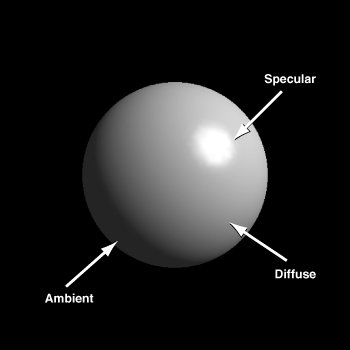
\includegraphics[width=200pt]{img/light}
    \caption{Lighting in OpenGL}
    \label{fig:lighting}
  \end{center}
\end{figure}

Ambient light simulates indirect lighting. It illuminates all 
geometry in a scene at the same intensity.
\\
Diffuse light illuminates a surface based on its orientation 
to a light source. OpenGL diffuse lighting adheres to 
Lambert's law, in which the amount of illumination is proportional 
to the cosine of the angle between the surface normal and the 
light vector, and the diffused light reflects equally in 
all directions.
\\
Specular light approximates the reflection of the light source on 
a shiny surface.
\\
At first glance, controlling OpenGL lighting might appear complex. 
The amount of code required to obtain simple lighting effects, 
however, is actually quite small. That is:

\begin{lstlisting}[caption={Lighting example}, label={code:lighting}, frame=trBL]
// Enable OpenGL lighting
glEnable( GL_LIGHTING );

// Enable a single light source
glEnable( GL_LIGHT0 );
\end{lstlisting}

\texttt{GL\_LIGHT0} is one of the light points available to 
OpenGL programmers. For every light point, one can set its 
position and parameters for each light component. For example:

\begin{lstlisting}[caption={Complex lighting example}, label={code:complexlighting}, frame=trBL]
GLfloat lightpos[] = { 0.0f, 0.0f, 1.0f, 0.0f };
GLfloat lightcolor[] = { 1.0f, 1.0f, 1.0f };
GLfloat ambcolor[] = { 1.0f, 1.0f, 1.0f };

glEnable(GL_LIGHTING);
glEnable(GL_LIGHT0);                        
glLightfv(GL_LIGHT0, GL_POSITION, lightpos);
glLightfv(GL_LIGHT0, GL_AMBIENT, lightcolor);
glLightfv(GL_LIGHT0, GL_DIFFUSE, lightcolor);
glLightfv(GL_LIGHT0, GL_SPECULAR, lightcolor);
\end{lstlisting}
